\documentclass[psamsfonts,reqno]{amsart}

%-------Packages---------
\usepackage{amssymb,amsfonts}
\usepackage[all,arc]{xy}
\usepackage{enumerate}
\usepackage{mathrsfs}
\usepackage{graphicx}			% Insert images
\usepackage{algorithm}			% Algorithms/pseudocode
\usepackage{algpseudocode}		% Pseudocode
\usepackage{minted}				% Code highlighting
\usepackage{biblatex}			% To create bibliography
\addbibresource{citation.bib}	% Citation reference for bibliography
\usepackage[group-separator={\,}]{siunitx} 	% Formatting numbers (use spaces, not commas)
\newcommand{\Mod}[1]{\ (\mathrm{mod}\ #1)}

%--------Theorem Environments--------
%theoremstyle{plain} --- default
\newtheorem{thm}{Theorem}[section]
\newtheorem{cor}[thm]{Corollary}
\newtheorem{prop}[thm]{Proposition}
\newtheorem{lem}[thm]{Lemma}
\newtheorem{conj}[thm]{Conjecture}
\newtheorem{quest}[thm]{Question}

\theoremstyle{definition}
\newtheorem{defn}[thm]{Definition}
\newtheorem{defns}[thm]{Definitions}
\newtheorem{con}[thm]{Construction}
\newtheorem{exmp}[thm]{Example}
\newtheorem{exmps}[thm]{Examples}
\newtheorem{notn}[thm]{Notation}
\newtheorem{notns}[thm]{Notations}
\newtheorem{addm}[thm]{Addendum}
\newtheorem{exer}[thm]{Exercise}

\theoremstyle{remark}
\newtheorem{rem}[thm]{Remark}
\newtheorem{rems}[thm]{Remarks}
\newtheorem{warn}[thm]{Warning}
\newtheorem{sch}[thm]{Scholium}

\makeatletter
\let\c@equation\c@thm
\makeatother
\numberwithin{equation}{section}

\bibstyle{plain}

%--------Meta Data: Fill in your info------
\title{Large Integer Multiplication:\\A Friendly Introduction\\to Select Multiplication Algorithms}

\author{JT Miller}

\date{December 8, 2023}

\begin{document}

\begin{abstract}

How do computers multiply integers larger than the number of bits within dedicated hardware? This paper provides a survey of several large integer multiplication algorithms that answer this question. The aim of the paper is to provide a friendly introduction with many examples such that undergraduate students can look past the complexity of these algorithms, grasp the fundamentals, and hopefully understand some of the beauty and wonder in the algorithms. 

\end{abstract}

\maketitle

\tableofcontents

\section{Introduction}

Large integer multiplication is pervasive in our lives in the form of cryptography. One need only look at the innards of any crypto library to find a BigInt library or API behind the scenes. Within those libraries/APIs are the algorithms discussed within this paper. There are other less pervasive uses, such as scientific and algorithm research, large-scale data analysis, and of course computational mathematics. 

How do computers multiply integers larger than the number of bits within dedicated hardware? This paper provides a survey of several large integer multiplication algorithms that answer this question. The aim of the paper is to provide a friendly introduction with many examples such that undergraduate students can look past the complexity of these algorithms, grasp the fundamentals, and hopefully understand some of the beauty in the algorithms. 

The title of the paper is a tribute to Dr. Silverman's wonderful \textit{A Friendly Introduction to Number Theory}. We will start with grade school multiplication, then cover a simple but useful extension that allows multiplication in "chunks". We then cover the first advance in nearly 4000 years \cite{burton1985history}, Karatsuba's algorithm. Next we will discuss the Toom Cook algorithm that is a generalization of Karatsuba's algorithm. Next we cover the fundamentals of the Discrete Fourier Transform (DFT) and Fast Fourier Transform (FFT) to understand how these algorithms are used to multiply large integers. Finally, we cover the Sch\"{o}nhage-Strassen multiplication algorithm, which gets us to $\mathcal{O}(n \log n \log \log n)$ time complexity.

\section{Grade School Multiplication}
Multiplication dates back to at least 2000 B.C. \cite{burton1985history} and of course we all learn how to multiply integers in grade school. A review of this algorithm gives us a grasp of the terminology and notation we will use throughout the rest of this paper to discuss multiplication algorithms. We start with a representation for integers, which will be useful for later algorithms.

\subsection{Integer Representation \nopunct}

We can express any positive integer $x$ as a summation of coefficients raised to a base power \cite{silverman2014friendly}:
\begin{equation}
	x = \sum_{i=0}^{n-1} X_iB^i.
\end{equation}
Given a base system and coefficients, we can express $x$ as a coefficient vector with $n$ entries: 
\begin{equation}
	\mathbf{X}=\{X_0, X_1, X_2, ..., X_{n-1}\}.
\end{equation}
E.g. we can represent the number $40342$ as 
\begin{equation}
	\mathbf{X}=\{2, 4, 3, 0, 4\}
\end{equation}
and in base 10 we would have 
\begin{equation}
	2 \cdot 10^0 + 4 \cdot 10^1 + 3 \cdot 10^2 + 0 \cdot 10^3 + 4 \cdot 10^4 =40342.
\end{equation}

Note that our coefficients for powers appear "backward" in the set/array, as lower-powered coefficients appear first, but we naturally write higher-power to lower-power coefficients left to right when expressing numbers. Even from this simple idea, we can make a few observations that will prove useful later. Given two positive integers $x$ and $y$, with one integer having fewer coefficients, we can still express the integers as vectors of the same length by zero-padding the smaller integer. E.g. let $x=389$ and $y=4$, then we can simply say $\mathbf{X}=\{9, 8, 3\}$ and $\mathbf{Y}=\{4, 0, 0\}$. If the larger integer has $n$ coefficients, we now have two integers with $n$ coefficients.

How many coefficients are necessary to store the result of two $n$-digit positive integers? 
\begin{lem}
	Multiplying two $n$-digit positive integers requires no more than $2n$ coefficients. 
\end{lem}
\begin{proof}
	Let $x$ be an $n$-digit positive integer in positive base $B$. 
	\begin{align}
		x & \leq B^n-1 \\
		x^2 & \leq ({B^n-1})^2 \\
		x^2 & \leq B^{2n} - 2B^n + 1 \label{max_base_number}
	\end{align}
	$2B^n > 1$ for all $B>0$, so we may simplify the right side of equation~\ref{max_base_number} to 
	\begin{align}
		x^2 & < B^{2n}
	\end{align}
\end{proof}
Let's work an example multiplying $9999 \times 9999 = 99980001$ in base 10. We have $B=10$ and $n=4$. In this case, we are using the maximum value ($9999$) that can be represented in base 10 with 4 digits. We can simply use equation~\ref{max_base_number} directly and compute $x^2$.
\begin{align*}
	x^2 &= B^{2n} - 2B^n + 1 \\
	x^2 &= 10^8 - 2 \cdot 10^4 + 1 \\
	x^2 &= 99980001
\end{align*}

Let us now discuss our (modified) grade school multiplication algorithm.

\subsection{Algorithm \nopunct}

For grade school multiplication, let us use the values $x=123$ and $y=789$ to illustrate our algorithm. Instead of simply multiplying the ones' digits $9$ and $3$ and writing the new ones' digit $7$ and carrying the $2$, we will write the individual products in each "column" corresponding to the base power, as shown in Figure~\ref{fig:gs01}. After we have computed all partial products, we add the partial products within each "column" or base power. Finally, we carry any overflow of partial products to the next column/base power, and we have our summation of final products yielding the answer $97047$. 
\begin{figure}[h]
	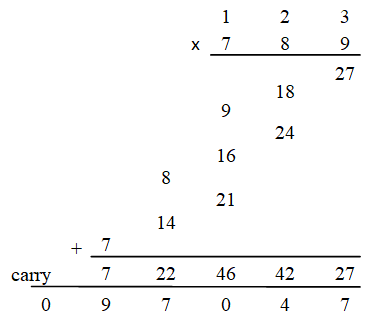
\includegraphics{img/gs_multiplication_ex_01}
	\caption{Grade School Multiplication of $123 \times 789$}
	\label{fig:gs01}
\end{figure}

Expressed mathematically, we are performing the following,
\begin{equation}
	\label{gsmul}
	xy = \sum_{k=0}^{n-1}\sum_{j=0}^{n-1}X_jY_kB^{j+k}.
\end{equation}

Now, let us determine an algorithm for performing our grade school multiplication. 

\begin{algorithm}
	\caption{Grade School Multiplication}
	\label{gs_mult_algo}
	\begin{algorithmic}
	\For{$j \in \{0,1,...,n-1\}$}
		\For{$k \in \{0,1,...,n-1\}$}
			\State {$W[j+k] += X_jY_kB^{j+k}$}
		\EndFor
	\EndFor
	\State $c = 0$
	\For{$j \in \{0,1,...,2n-2\}$}
		\State $c = W[j] \Mod{B}$				
		\State $W[j] = \lfloor W[j] / B \rfloor$
		\State $W[j+1] += c$
	\EndFor
	\State return $W$
\end{algorithmic}
\end{algorithm}

\subsection{Time Complexity Analysis \nopunct}

We will not belabor the time-complexity analysis to determine exact counts of the operations involved. In general additions are easier for computers, so we will typically only care about the number of necessary multiplications. From Figure~\ref{fig:gs01} we can see that for $n$ digits, we have $n \times n$ partial products to compute. Accordingly, our grade school multiplication algorithm yields $\mathcal{O}(n^2)$.

\subsection{Code Examples \nopunct}

\begin{minted}{python}
def left_to_right(x: list[int]) -> str:
    """Take a least significant first digit set and return a string representation
    of the number."""
    return "".join(str(d) for d in x[::-1])
    
def zero_pad(x: list[int], n: int, pad: int=0) -> list[int]:
    """Zero pad a list to the given length."""
    return [pad] * (n - len(x)) + x

def grade_school_multiplication(X: list[int], Y: list[int]) -> list[int]:
    # Pad the shorter list with zeros to match the lengths
    n = max(len(X), len(Y))
    X = zero_pad(X, n)
    Y = zero_pad(Y, n)

    # Initialize the result list W with zeros, length should be 2 * n
    W = [0] * (2 * n)

    # Multiply all partial products and add them to W
    for j in range(len(X)):
        for k in range(len(Y)):
            W[j + k] += X[j] * Y[k]

    # Handle carries from least significant to most significant digit
    for i in range(len(W) - 1):
        carry, W[i] = divmod(W[i], 10)
        W[i + 1] += carry

    # Remove excess leading zeros, if any, but leave at least one digit
    while len(W) > 1 and W[-1] == 0:
        W.pop()

    return W
\end{minted}

\section{Chunky Grade School Multiplication}

We can make a simple modification to our grade school multiplication that allows us to increase our multiplication speed by a factor of our machine's bit-length. Because this technique is generic, the exact bit-lengths involved in integer hardware multiplication aren't necessarily important. The increase comes by recognizing that instead of multiplying a single digit at a time, we can multiply chunks of digits. We will use $\num{123456} \times \num{987654} = \num{121931812224}$ to illustrate\footnote{Note that the spaces in numbers such as these are strictly for readability purposes. Numbers formatted with spaces like those in the previous multiplication are still single contiguous numbers.} our chunky grade school multiplication algorithm improvement.

Figure~\ref{fig:cgs01} shows how we can group our digits into chunks. These chunks allow fewer partial products even though we now have more total digits. The chunks "skip" base powers by grouping digits. 
 
\begin{figure}[h]
	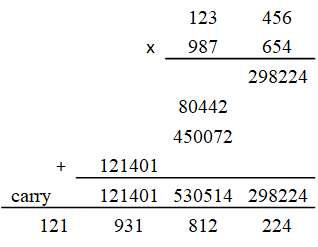
\includegraphics{img/chunky_gs_mul_ex_01}
	\caption{Chunky Grade School Multiplication of $\num{123456} \times \num{987654}$}
	\label{fig:cgs01}
\end{figure}

If we group 3 digits then we are using a chunk size of 3 base powers, which we then keep track of throughout the algorithm. In actual large integer multiplication algorithms, we must be careful to guarantee that the summation of partial products for a given base power/column fits within the machine word size/bit width. Let us use the positive integer $h$ for chunk size, then we have just a small modification from equation~\ref{gsmul}, 

\begin{equation}
	xy = \sum_{k=0}^{n-1}\sum_{j=0}^{n-1}X_jY_kB^{h(j+k)}.
\end{equation}

\subsection{Algorithm \nopunct}

\begin{algorithm}
	\caption{Chunkify}
	\label{chunkify}
	\begin{algorithmic}
		\State Pick a chunk size $h > 1$
		\State Pad $X, \; Y$ to $kh$ where $k$ is a positive integer
		\State $n = len(X)/h$
		\State $X_{chunky} = \{0, 0, ..., 0\}$
		\State $Y_{chunky} = \{0, 0, ..., 0\}$
		\For{$j \in \{0,1,...,nh-1\}$}
			\State $X_{chunky}[\lfloor j/h \rfloor] += X[j] * 10^{j \Mod{h}}$
			\State $Y_{chunky}[\lfloor j/h \rfloor] += X[j] * 10^{j \Mod{h}}$
		\EndFor
		\State return $X_{chunky}, \; Y_{chunky}$
	\end{algorithmic}
\end{algorithm}

\begin{algorithm}
	\caption{Chunky Grade School Multiplication}
	\label{chunky_gs_mult_algo}
	\begin{algorithmic}
		\For{$j \in \{0,1,...,n-1\}$}
			\For{$k \in \{0,1,...,n-1\}$}
				\State {$W[j+k] += X_jY_kB^{j+k}$}
			\EndFor
		\EndFor
		\State $c = 0$
		\For{$j \in \{0,1,...,2n-2\}$}
			\State $c = W[j] \Mod{B^h}$				
			\State $W[j] = \lfloor W[j] / B^h \rfloor$
			\State $W[j+1] += c$
		\EndFor
		\State return $W$
	\end{algorithmic}
\end{algorithm}

\subsection{Time Complexity Analysis \nopunct}

From Figure~\ref{fig:cgs01} we can see that we have reduced from $n \times n$ operations to $n/h \times n/h$ operations, which can be a significant real reduction, but still results in a run time of $\mathcal{O}(n^2)$.

\subsection{Code Examples \nopunct}

\begin{minted}{python}
def chunkify(x: list[int], h: int) -> list[int]:
    """Split a list into chunks of size n."""
    if len(x) % h != 0:
        raise ValueError(f"Length of list must be a multiple of {h}, \
        	{len(x)} is not!")
    n = len(x) // h
    chunks = [0] * n
    for ix, val in enumerate(x):
        chunks[ix // h] += val * 10 ** (ix % h)
    return chunks


def chunky_grade_school_multiplication(
	X: list[int], Y: list[int], h: int
) -> list[int]:
    # Pad the shorter list with zeros to match the lengths
    n = max(len(X), len(Y))
    X = zero_pad(X, n)
    Y = zero_pad(Y, n)

    # Verify X and Y are chunkable
    if len(X) % h != 0:
        raise ValueError(f"Length of X must be a multiple of {h}, \
        	{len(X)} is not!")

    # Chunkify X and Y
    X = chunkify(X[:], h)
    Y = chunkify(Y[:], h)

    n = len(X_chunks)

    # Initialize the result list W with zeros, length should be 2 * n
    W = [0] * (2 * n)

    # Multiply all partial products and add them to W
    for j in range(len(X)):
        for k in range(len(Y)):
            W[j + k] += X[j] * Y[k]

    # Handle carries from least significant to most significant digit
    for i in range(len(W) - 1):
        carry, W[i] = divmod(W[i], 10**h)
        W[i + 1] += carry

    # Remove excess leading zeros, if any, but leave at least one digit
    while len(W) > 1 and W[-1] == 0:
        W.pop()

    return W
\end{minted}

\section{Karatsuba}
We now turn our attention to Karatsuba's algorithm. In 1960, Andrey Kolmogorov conjectured that $\mathcal{O}(n^2)$ was as fast as multiplication could be achieved. Kolmogorov held a seminar at Moscow University where he presented this and other conjectures. Anatoly Karatsuba, a 23-year-old student, found a divide and conquer deconstruction method that multiplies integers in $\mathcal{O}(n^{\log_2 3})$ that he presented at the next seminar, which Kolmogorov then disbanded (TODO: INSERT REFERENCE HERE). Kolmogorov was so impressed with Karatsuba's algorithm that he wrote a paper for him, which Karatsuba only became aware of after the edits were mailed back to him \cite{karatsuba1995complexity}. Perhaps the best way to motivate some is to say that something is impossible.

\subsection{Algorithm \nopunct}
Karatsuba's algorithm involves manipulating the partial products involved in multiplication, a divide and conquer approach. Let the tens' and ones' digits of $x$ to be $ab$, or $X_1 = a$, and $X_0 = b$ from our previous discussions. Similarly, let the tens and ones' digits of $y$ be $cd$, or $Y_1 = c$ and $Y_0 = d$. Figure~\ref{fig:gs_abcd} shows this simple grade school multiplication. 

\begin{figure}[h]
	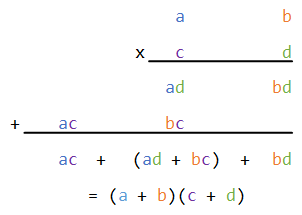
\includegraphics{img/gs_abcd}
	\caption{Grade School $abcd$ Multiplication}
	\label{fig:gs_abcd}
\end{figure}

Note that we are neglecting the base. Figure~\ref{fig:gs_abcdz} shows the same multiplication with our base $z$ included. 

\begin{figure}[h]
	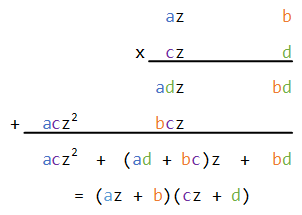
\includegraphics{img/gs_abcdz}
	\caption{Grade School $abcdz$ Multiplication (includes base $z$)}
	\label{fig:gs_abcdz}
\end{figure}

Karatsuba recognized that the multiplication of partial products, $(a+b)(c+d)=ac+(ad+bc)+bd$ could be manipulated to yield three multiplications instead of four. $ac$ is one multiplication, $bd$ is the second, and then we can use the fact that $(ad+bc) = (a+b)(c+d) - (ac + bd)$ for the third multiplication. We now have all the partial products necessary, having deconstructed the addition of partial products. At the cost of a few more additions and subtractions, we can remove one multiplication. Figure~\ref{fig:abcd_equation} shows this simple coefficient manipulation with the multiplications numbered at the bottom of equations and the "free" multiplication shown.

\begin{figure}[h]
	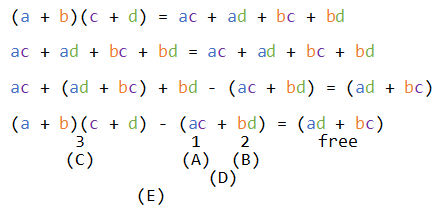
\includegraphics{img/abcd_equation}
	\caption{Karatsuba's Manipulation of Coefficients}
	\label{fig:abcd_equation}
\end{figure}

Figure~\ref{fig:karatsuba_example} shows an example for $\num{25786109} \times \num{72166948} = \num{1860904787325332}$ with the same coloring used to denote $abcd$ as the previous explanations. Note that we have combined the algorithm with chunking (typically this is referred to as blocking, but the term chunking is more fun) that combines several coefficients. 

\begin{figure}[h]
	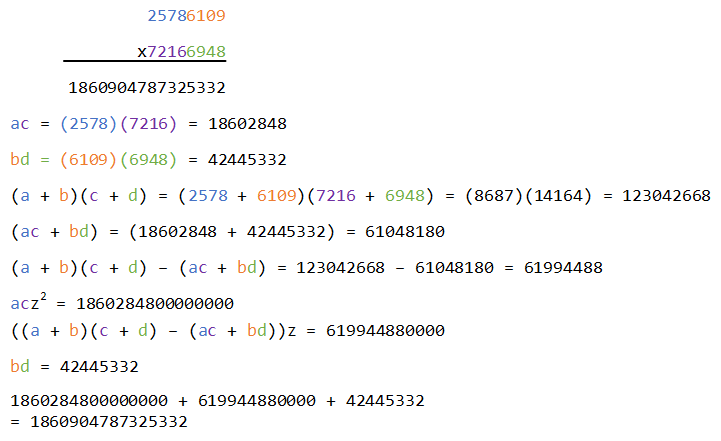
\includegraphics{img/karatsuba_example}
	\caption{Karatsuba Example}
	\label{fig:karatsuba_example}
\end{figure}

Karatsuba's three coefficient products, $ac$, $bd$, and $(a+b)(c+d)$, can be used to recursively subdivide the problem further. Although not necessary (we could have used more coefficients and a larger base power), Figure~\ref{fig:karatsuba_large_example} shows a larger Karatsuba example where we recursively apply Karatsuba to coefficients. Note that we dispense with the summation of partial products after the first stage as the quantities become cumbersome to print. 

\begin{figure}[h]
	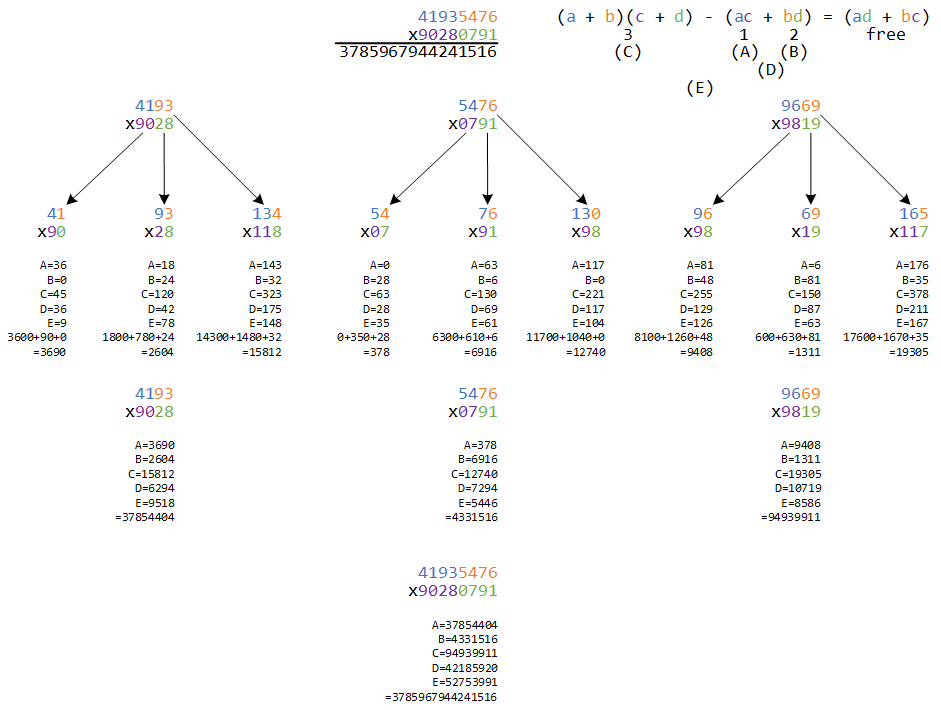
\includegraphics{img/karatsuba_large_example}
	\caption{Larger Karatsuba Example}
	\label{fig:karatsuba_large_example}
\end{figure}

(TODO: Add algorithm)

\subsection{Time Complexity Analysis \nopunct}

As we noted above, because Karatsuba allows recursively subdividing the problem in half, using three coefficient multiplications, the runtime is $\mathcal{O}(n^{\log_2{3}})$. $\log_2{3} \approxeq 1.585$, so the runtime complexity of Karatsuba's algorithm is commonly referred to as $\mathcal{O}(n^{1.585})$. 

\subsection{Code Examples \nopunct}

(TODO: Add python for real algorithm and discussion)

\begin{minted}{matlab}
function [] = karatsuba(x, y, n)
	a = floor(x/10^n);
	b = mod(x,10^n);
	c = floor(y/10^n);
	d = mod(y,10^n);
	
	A = a*c;
	B = b*d;
	C = (a+b)*(c+d);
	D = A+B;
	E = C - D;
	result = A*10^(2*n) + E*10^n + B;
	fprintf("A=%d\n", A);
	fprintf("B=%d\n", B);
	fprintf("C=%d\n", C);
	fprintf("D=%d\n", D);
	fprintf("E=%d\n", E);
	fprintf("%d+%d+%d\n", A*10^(2*n), E*10^n, B);
	fprintf("=%d\n\n", result);
end	
\end{minted}

\section{Toom Cook}

\subsection{Algorithm \nopunct}
\subsection{Time Complexity Analysis \nopunct}
\subsection{Code Examples \nopunct}

\section{The DFT and FFT}

\subsection{Algorithm \nopunct}
\subsection{Time Complexity Analysis \nopunct}
\subsection{Code Examples \nopunct}

\section{Multiplication via the Complex FFT}

\subsection{Algorithm \nopunct}
\subsection{Time Complexity Analysis \nopunct}
\subsection{Code Examples \nopunct}

\section{Modulo Arithmetic}

\section{Sch\"{o}nhage-Strassen}

\subsection{Algorithm \nopunct}
\subsection{Time Complexity Analysis \nopunct}
\subsection{Code Examples \nopunct}

\section{O(n log n)}

\section{Conclusion}

\section*{Acknowledgments} I would like to extend my heartfelt thanks to Dr. Huang for allowing me to pursue an open-ended research topic and providing guidance and motivation along the way. I am aware that undergraduate research has few tangible benefits for a professor, but this has been a tremendously rewarding experience for me. Thank you for patience during the weeks where I was making no visible progress. Thank you for your mentorship and gentle steering during this research. Most of all, thank you for sharing your passion for algorithms and mathematics. That passion is infectious and has made working with you not just a rewarding, but joyful experience. 

\printbibliography

\end{document}

